%%%%%%%%%%%%Outline%%%%%%%%%%%%%%%%%%

%%%
% message<eBPF reaches the kernel through a compile, verify, JIT pipeline>
% every eBPF program reaches the kernel through the pipeline
% a user-space compiler compiles source to bytecode
% the kernel verifies, JIT-compiles, and attaches the program
% the attached program runs at each hook invocation

%%%
% message<the compiler can emit only operations the eBPF instruction set defines>
% an eBPF program reaches the kernel as compiler-produced bytecode
% a front-end lowers source code to LLVM IR
% the middle-end runs its optimization passes
% the eBPF backend lowers IR to restricted bytecode

%%%
% message<the verifier checks safety over a fixed opcode set>
% the verifier statically checks every program for safety
% the analysis uses abstract interpretation
% each defined opcode has its own abstract semantics
% unknown opcodes are rejected, so a new opcode needs new semantics
% the verifier also does targeted rewrites before the JIT

%%%
% message<the JIT translates one instruction at a time without cross-instruction optimization>
% the eBPF JIT compiler translates verified bytecode to machine code
% translation proceeds one instruction at a time with fixed registers
% within-instruction encoding choices apply per instruction
% multiple passes stabilize the jump encodings
% the JIT performs no cross-instruction optimization

%%%
% message<Section 3 measures the performance of the machine code the pipeline produces>
% Section 3 measures the performance of the machine code the pipeline produces

%%%%%%%%%%%%Outline%%%%%%%%%%%%%%%%%%

\section{The eBPF Compilation Pipeline}
\label{sec:background}

Every eBPF program reaches the kernel through the eBPF compilation pipeline, shown in Figure~\ref{fig:ebpf}. A user-space compiler compiles source code to eBPF bytecode. The kernel then verifies the bytecode, JIT-compiles the verified bytecode to machine code, and attaches the compiled program to a hook point (e.g., XDP, tc). Once attached, the program runs each time the kernel invokes the hook.

\begin{figure}[t]
  \centering
  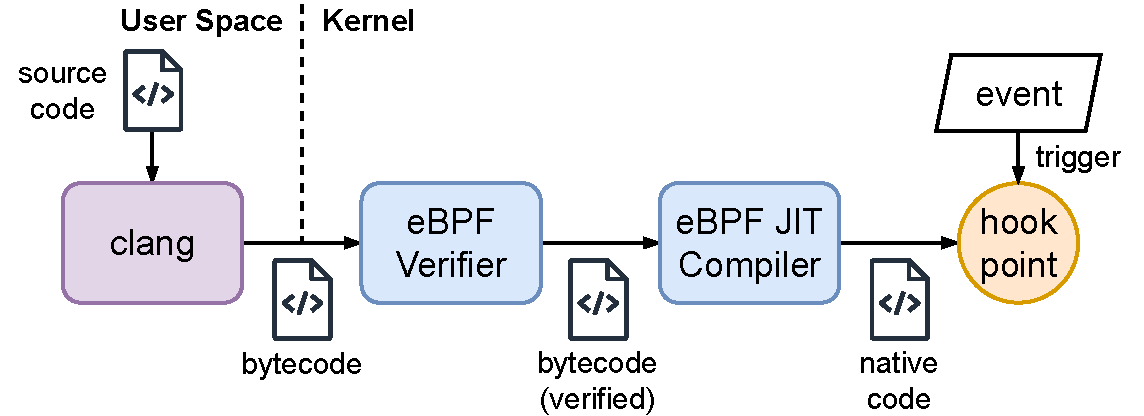
\includegraphics[width=\linewidth]{figures/sec-2-ebpf-pipeline.pdf}
  \caption{The eBPF execution pipeline.}
  \label{fig:ebpf}
\end{figure}

\noindent\textbf{Source compilation.}
An eBPF program reaches the kernel as bytecode produced by a user-space compiler. A language-specific front-end (e.g., Clang for C) lowers source code to LLVM IR. LLVM's middle-end runs its optimization passes. The LLVM eBPF backend lowers the optimized IR to eBPF bytecode, restricted to operations the eBPF instruction set defines.

\noindent\textbf{Verification.}
The eBPF verifier statically checks every loaded program for safety, proving properties such as memory safety, termination, and absence of uninitialized reads. The analysis uses abstract interpretation~\cite{gershuni2019simple}. Each of the 117 opcodes the eBPF instruction set defines~\cite{rfc9669} has its own abstract semantics. Unknown opcodes are rejected, so adding an opcode requires defining new semantics. After safety analysis succeeds, the verifier also performs a few targeted bytecode rewrites (e.g., dead-code elimination) before passing the program to the JIT.

\noindent\textbf{JIT compilation.}
The eBPF JIT compiler translates the verified bytecode into machine code. The translation proceeds one instruction at a time, with eBPF registers \texttt{r0}--\texttt{r10} mapped to fixed native registers on each target architecture. Encoding-level optimizations within each instruction include selecting the shortest immediate encoding, choosing short jumps when the offset fits, and emitting prologue push/pop instructions only for callee-saved registers the program uses. Multiple passes iterate until jump encodings stabilize. The JIT performs no cross-instruction optimization (e.g., global register allocation, instruction scheduling).

% \S\ref{sec:characterization} measures the performance of the machine code the pipeline produces.